\chapter{De afweer}\label{ch:g9:immune-defenses}

De deuren worden gehouden
(\cref{prop:g9:microbes-and-infection:doors}) --- en toch landt er
soms een indringer: de \omterm{def:g9:microbes-and-infection:sorted}{bacteriën} van de splinter die zich in het
warme weefsel vermeerderen, het \omterm{def:g9:microbes-and-infection:sorted}{virus} dat al in de cellen van de
luchtweg drukt. Wat er daarna gebeurt, is het derde grote stelsel
van het lichaam na de \omterm{def:g5:brain-in-command:system}{zenuwen} en de \omterm{def:g8:hormonal-communication:glands}{hormonen}: de afweer --- een
staand leger, een korps specialisten met geheugen, en de truc van
de vaccinatie die het vooraf traint.

\section{De snelle reactie: ontsteking}

\begin{definition}[Het staande leger]\label{def:g9:immune-defenses:standing}
Door het \omterm{prop:g4:journey-of-food:absorb}{bloed} en de weefsels patrouilleren de witte
bloedcellen\index{witte bloedcel} --- de troepen van de afweer, in
het beenmerg gemaakt, rijdend over het netwerk van
\cref{prop:g4:heart-and-blood:carries}. De eerste hulpverleners
zijn de \emph{opslokkers}: cellen die om een indringer heen
stromen en hem verteren (de stromende klodder van
\cref{ex:g6:cell-unit-of-life:drop} voerde dezelfde manoeuvre uit
als een vrijlevende jager --- het lichaam zet de eeuwenoude truc
als verdediging in).
\end{definition}

\begin{proposition}[Ontsteking, goed gelezen]\label{prop:g9:immune-defenses:inflammation}
De nasleep van een splinter --- roodheid, warmte, zwelling,
kloppen --- is niet de \omterm{def:g9:microbes-and-infection:stages}{infectie} die wint, maar de verdediging die
aankomt. Alarmsignalen uit het beschadigde weefsel verwijden de
plaatselijke vaten (het omleiden uit
\cref{prop:g7:organs-at-work:supply}, gevorderd): meer warm \omterm{prop:g4:journey-of-food:absorb}{bloed},
lekker gemaakte wanden, opslokkers die zich uit de \omterm{def:g7:heart-and-circulation:vessels}{haarvaten}
persen en naar de plek kruipen en onderweg \omterm{def:g9:microbes-and-infection:sorted}{bacteriën} opeten. Pus is
de balans van het slagveld --- opgebruikte opslokkers, dode
indringers, gruis. De meeste landingen eindigen hier, in dagen,
onopgemerkt.
\end{proposition}
\admitted

\begin{example}[Een genezende snee lezen]\label{ex:g9:immune-defenses:cut}
Dag één: een rode, warme, gevoelige kring --- de vaten wijd, de
troepen komen aan. Dag twee: een beetje pus --- de balans. Dag
vier: de kring vervaagt, de korst is droog --- de vermeerdering
verloor de race van het opslokken, en de heropbouw van de \omterm{def:g1:the-five-senses:sense}{huid}
(\cref{prop:g5:first-look-at-cells:growth}) sluit de deur achter de
oorlog. De hele veldtocht, gestreden en gewonnen onder de schaal
van de zorgen.
\end{example}

\section{De specialisten: herkenning en geheugen}

\begin{proposition}[De specifieke reactie]\label{prop:g9:immune-defenses:specific}
Als de snelle reactie wordt ingehaald, betreedt het korps
specialisten het veld --- langzamer, en nauwkeurig:
\begin{itemize}
  \item elke indringer draagt merktekens op zijn oppervlak --- zijn
        \emph{antigenen}\index{antigeen} --- moleculaire vormen
        die de specialisten als vreemd lezen (de zelfmerktekens
        van \cref{ex:g9:unique-individuals:medicine} zijn hetzelfde
        lezen, naar binnen gericht);
  \item onder de gespecialiseerde witte cellen dragen er enkele
        ontvangers die op \emph{dit} antigeen passen; het contact
        selecteert hen, en ze vermeerderen zich tot een
        kloonleger (de logica van de selectie, binnen het lichaam
        in dagen uitgevoerd);
  \item hun wapens: \emph{antistoffen}\index{antistof} --- passend
        gemaakte moleculen die in het \omterm{prop:g4:journey-of-food:absorb}{bloed} gegoten worden en de
        indringer voor de opslokkers vastpinnen en samenklonteren
        --- en dodende specialisten die de eigen gekaapte cellen
        van het lichaam vernietigen, de enige manier om de
        drukpersen van een \omterm{def:g9:microbes-and-infection:sorted}{virus} te stoppen
        (\cref{ex:g9:microbes-and-infection:contrast});
  \item de kosten van het gevecht horen bij de ziekte: de koorts
        (een lichaam dat met opzet heet draait --- veel
        \omterm{prop:g9:microbes-and-infection:mostly}{ziekteverwekkers} vermeerderen zich warm slechter), de pijn
        in het lijf, en de gezwollen \emph{lymfeklieren} --- de
        kazernes van de specialisten, overvol in oorlogstijd.
\end{itemize}
\end{proposition}
\admitted

\begin{definition}[Afweergeheugen]\label{def:g9:immune-defenses:memory}
Na de overwinning trekt een deel van het kloonleger zich terug als
\emph{geheugencellen}\index{geheugencel}: langlevende specialisten
die de beschrijving van het antigeen vasthouden. Een tweede landing
van \emph{dezelfde} indringer treft een voorbereid korps ---
reactie in uren, de indringer opgeruimd nog voor de verschijnselen:
je bent \emph{immuun}\index{immuniteit}. Eén keer mazelen, nooit
twee keer; de stam van vorige winter die de uitbraak van dit jaar
niet opnieuw kon ontsteken
(\cref{pb:g9:microbes-and-infection:1}). Het geheugen is de reden
dat dezelfde verkoudheid nooit twee keer lijkt te komen --- en de
reden dat verkoudheden blijven komen: hun \omterm{def:g9:microbes-and-infection:sorted}{virussen} muteren snel
(\cref{prop:g9:genes-and-dna:explains}) naar beschrijvingen die het
geheugen niet bezit.
\end{definition}

\section{De verdediging trainen: vaccinatie}

\begin{proposition}[Vaccinatie]\label{prop:g9:immune-defenses:vaccination}
\emph{Vaccinatie}\index{vaccinatie} is afweergeheugen dat zonder de
ziekte gemaakt wordt: bied de specialisten de \emph{beschrijving}
van de indringer aan --- gedode of verzwakte \omterm{def:g6:producing-our-food:fermentation}{microben},
onschadelijke fragmenten die het antigeen dragen --- en het hele
programma van selectie en geheugen loopt af, zonder het gevaar. Het
getrainde korps ontmoet de echte ziekteverwekker daarna, als het er
ooit van komt, als een tweede landing. Twee gevolgen dragen het
gewicht voor de volksgezondheid:
\begin{enumerate}
  \item wie gevaccineerd is, is beschermd nog vóór het eerste
        gevecht --- doorslaggevend bij ziekten waarvan het eerste
        gevecht kan doden of verminken;
  \item genoeg gevaccineerde buren hongeren een uitbraak uit door
        gebrek aan vatbare gastheren (het uitdoven van
        \cref{pb:g9:microbes-and-infection:1}): de bescherming
        bundelt zich --- het schild dekt wie te jong of te ziek
        zijn om zelf getraind te worden.
\end{enumerate}
\end{proposition}
\admitted

\begin{example}[Van de gok met de koepokken tot de uitroeiing]\label{ex:g9:immune-defenses:history}
De geschiedenis loopt van de gok van Jenner in 1796 ---
melkmeisjes kregen milde koepokken en nooit pokken; een enting met
koepokken trainde tegen de moordenaar --- via de doelbewuste
vaccins met verzwakte \omterm{def:g6:producing-our-food:fermentation}{microben} van Pasteur (de schrijver van
\cref{ex:g9:microbes-and-infection:history}, die zijn theorie
voltooide), tot het appèl van de twintigste eeuw: de pokken, de
oude gesel van de mensheid, \emph{uitgeroeid} --- het \omterm{def:g9:microbes-and-infection:sorted}{virus} sinds
het eind van de jaren zeventig \omterm{prop:g5:biodiversity:loss}{uitgestorven} in het wild --- en
polio teruggedrongen tot de laatste hoeken van de kaart. Getraind
geheugen, gebundeld, is het enige wapen dat ooit een menselijke
ziekte heeft uitgeroeid.
\end{example}

\begin{omfigure}
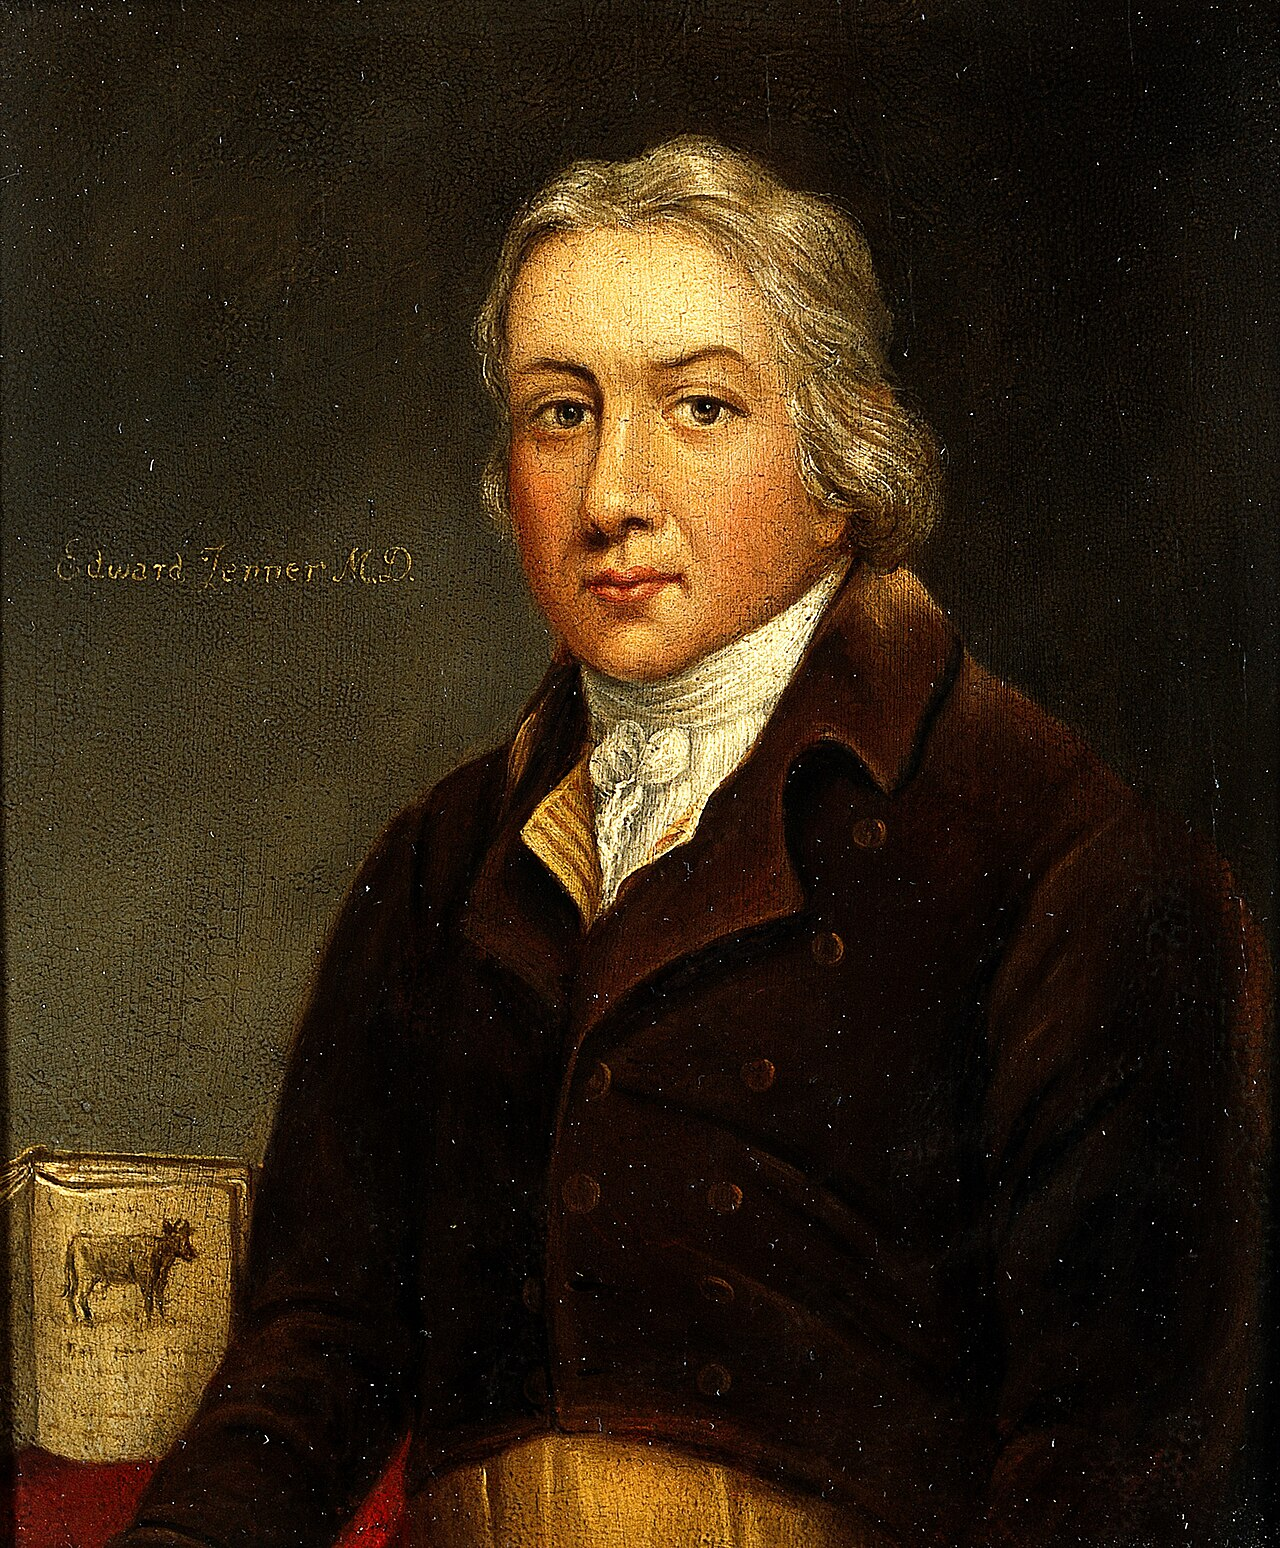
\includegraphics[width=0.46\linewidth]{images/book1/jenner.jpg}

{\small Edward Jenner, die in 1796 de gok met de koepokken waagde
die vaccinatie werd. Olieverfschilderij, Wellcome Collection,
CC~BY~4.0.}
\end{omfigure}

\begin{method}[Elke afweergebeurtenis lezen]\label{met:g9:immune-defenses:read}
Bij elke \omterm{def:g9:microbes-and-infection:stages}{infectie}, elk herstel, elk vaccin of elke testuitslag:
\begin{enumerate}
  \item bepaal de fase van de ontmoeting: eerste of tweede
        landing? (het geheugen verandert alles);
  \item noem de hulpverleners: de snelle reactie van de
        opslokkers, het kloonleger van de specialisten, of het
        staande geheugen;
  \item lees de tekenen goed: ontsteking en koorts als de
        verdediging aan het werk, gezwollen \omterm{def:g8:hormonal-communication:glands}{klieren} als kazernes;
  \item bepaal bij een vaccin welke beschrijving wordt
        aangeboden, en wiens bescherming het bundelt.
\end{enumerate}
\end{method}

\section{Oefeningen}

\begin{exercise}[$\star$]\label{exo:g9:immune-defenses:1}
Wie zijn het staande leger en de eerste hulpverleners, en waar
worden ze gemaakt?
\end{exercise}

\begin{exercise}[$\star$]\label{exo:g9:immune-defenses:2}
Vertaal de vier tekenen van de splinter in gebeurtenissen van de afweer.
\end{exercise}

\begin{exercise}[$\star$]\label{exo:g9:immune-defenses:3}
Wat is een antigeen, wat een antistof, en wat is het verband
ertussen?
\end{exercise}

\begin{exercise}[$\star$]\label{exo:g9:immune-defenses:4}
Waarom moeten dodende specialisten bij een virusinfectie de eigen
cellen van het lichaam vernietigen?
\end{exercise}

\begin{exercise}[$\star$]\label{exo:g9:immune-defenses:5}
Wat is een \omterm{def:g9:immune-defenses:memory}{geheugencel}, en wat treft een tweede landing aan?
\end{exercise}

\begin{exercise}[$\star$]\label{exo:g9:immune-defenses:6}
Definieer vaccinatie in één zin, opgebouwd uit ``beschrijving'' en
``geheugen''.
\end{exercise}

\begin{exercise}[$\star\star$]\label{exo:g9:immune-defenses:7}
Waarom is koorts een wapen en geen storing --- en welke eerdere
regel over \omterm{def:g6:exploring-our-environment:conditions}{omstandigheden} buit ze uit?
\end{exercise}

\begin{exercise}[$\star\star$]\label{exo:g9:immune-defenses:8}
``Eén keer mazelen, nooit twee keer --- en toch eeuwig
verkoudheden.'' Los beide helften op met
\cref{def:g9:immune-defenses:memory}.
\end{exercise}

\begin{exercise}[$\star\star$]\label{exo:g9:immune-defenses:9}
Het kloonleger van de specialisten is ``selectie, binnen het
lichaam uitgevoerd''. Breng de vergelijking in kaart op de drie
feiten van
\cref{prop:g9:how-species-change:selection}.
\end{exercise}

\begin{exercise}[$\star\star$]\label{exo:g9:immune-defenses:10}
Leg gebundelde bescherming uit --- en wie ervan afhangt --- met het
uitdoven van de uitbraak.
\end{exercise}

\begin{exercise}[$\star\star$]\label{exo:g9:immune-defenses:11}
Pas \cref{met:g9:immune-defenses:read} toe op: (a) een
tetanusherhalingsprik na de roestige spijker; (b) gezwollen \omterm{def:g8:hormonal-communication:glands}{klieren}
in de \omterm{def:g1:my-body:parts}{hals} bij een razende keelpijn.
\end{exercise}

\begin{exercise}[$\star\star\star$]\label{exo:g9:immune-defenses:12}
Schrijf de overlijdensadvertentie van de pokken zoals dit boek dat
zou doen: het mechanisme van het \omterm{def:g9:microbes-and-infection:sorted}{virus}, het getrainde geheugen dat
het in het nauw dreef, het bundelen dat het afmaakte --- en waarom
uitroeiing een uitsterven is (\cref{prop:g5:biodiversity:loss}) dat
voor één keer in het voordeel van de mensheid werkte.
\end{exercise}

\section{Probleem: Het vaccinatieregister}

\begin{problem}[{Weekendprobleem --- een week in een
gezondheidscentrum, met de afweermethode gelezen}]\label{pb:g9:immune-defenses:1}
Een (verzonnen) week in een gezondheidscentrum: maandag,
vaccinaties voor zuigelingen; dinsdag, de scheurwond van een boer
aan roestig draad en een herhalingsprik; woensdag, een geval van
mazelen bij een niet-gevaccineerd kind, en de contacten
nagelopen; donderdag, bloedtesten die het gehalte aan \omterm{prop:g9:immune-defenses:specific}{antistoffen}
aflezen; vrijdag, de jaarlijkse griepprikken voor het personeel.

\medskip\noindent\textbf{Deel I --- De gevallen van de week.}
\begin{enumerate}
  \item De zuigelingen van maandag krijgen druppels met verzwakte
        \omterm{def:g6:producing-our-food:fermentation}{microben} en injecties met fragmenten. Noem wat er wordt
        aangeboden, en welk programma in de weken erna
        afloopt.
  \item De boer van dinsdag: de scheurwond wordt schoongemaakt
        (welke verdedigingslinie?), en de herhalingsprik wordt
        gegeven. Wat doet een \emph{herhalingsprik} met een
        getraind geheugen --- en waarom laat juist tetanus geen
        gok op een eerste gevecht toe?
  \item Het mazelenkind van woensdag: eerste landing, volledig
        programma. Zet de ziekte op een tijdlijn: de snelle
        reactie ingehaald, het kloonleger opgezet, het herstel ---
        en wat er daarna terugtreedt.
  \item De nagelopen contacten vallen uiteen: gevaccineerden
        (onbezorgd), lang geleden genezenen (onbezorgd), en één
        niet-gevaccineerde zuigeling, angstig in de gaten
        gehouden. Lees elk met de eerste vraag van
        \cref{met:g9:immune-defenses:read}.
\end{enumerate}

\medskip\noindent\textbf{Deel II --- De metingen.}
\begin{enumerate}[resume]
  \item De testen van donderdag lezen het gehalte aan \omterm{prop:g9:immune-defenses:specific}{antistoffen}
        tegen doorgemaakte ziekten en vaccins af. Wat bevestigt
        een hoog gehalte, en welke celvoorraad impliceert het?
  \item Bij één patiënt is het gehalte jaren na de vaccinatie
        vervaagd, en er wordt een herhalingsprik voorgeschreven.
        Verklaar vervagen en opfrissen in termen van
        \omterm{def:g9:immune-defenses:memory}{geheugencellen}.
  \item Het griepvaccin van vrijdag is \emph{jaarlijks}, anders
        dan de programma's van maandag die één of twee keer
        lopen. Welke eigenschap van het griepvirus
        (\cref{def:g9:immune-defenses:memory}) dwingt de
        jaarlijkse hertraining af?
  \item Waarom vaccineert het centrum zijn \emph{personeel} met
        bijzondere nadruk? (Wiens bescherming bundelt zich waar,
        in een gebouw vol zieken en kwetsbaren?)
\end{enumerate}

\medskip\noindent\textbf{Deel III --- De betekenis van het
register.}
\begin{enumerate}[resume]
  \item De ouders van het niet-gevaccineerde mazelenkind hadden
        vaccins gevreesd en op ``natuurlijke'' eerste gevechten
        vertrouwd. Stel de zachtaardige rekensom van de arts op:
        vergelijk de kosten van de training met die van het eerste
        gevecht, voor mazelen.
  \item De in de gaten gehouden zuigeling was te jong voor het
        vaccin. Zeg wie hem hoorde te beschermen, en hoe die plicht
        in \cref{prop:g9:immune-defenses:vaccination} heet.
  \item Verbind dinsdag en woensdag met de twee historische namen
        uit \cref{ex:g9:immune-defenses:history}: wiens idee liep
        er in elk consult?
  \item Sluit het register af met de samenvatting van de week in
        één zin: wat het centrum feitelijk toedient, in de
        woordenschat van dit hoofdstuk.
\end{enumerate}
\end{problem}
